\subsection{Benötigte Kenntnisse}
Die Variable x=0-3.
Um das Programm zu erstellen werden Kenntnisse z.B. für die Timer CCU4x sowie deren Slices CC40-43 benötigt. Die Funktionen der CCU4x wird in der Reference Manuel beschrieben, siehe dazu Anhang, um die Timer zu Initialisieren wird die XMC LIb benötigt die eine fertige API mit bringt, siehe Kapitel Besonderheiten der Software, so wird nur noch die API mit den richtigigen Parametern beschrieben um die Timer lauffähig zu kriegen. 

\subsubsection{Durchgeführte Berechnungen}
Auch für die Programmierung waren diverse Berechnungen notwendig. So musste zur Erzeugung der Ultraschallimpulse ein Pulsweitenmoduliertes Rechteck signal geschaffen werden. Dafür wurde ein Timer der CCU4x auf einen Takt von 40kHz eingestellt. So musste bei eiem Timertakt von 96MHz eine Periodendauer von 2400 Takten, siehe unten die Berechnung und ein Compare-Wert von 1200 Takten eingestellt werden. Im Zählvorgang des Timers wird der Ausgang nach erreichen des Compare-Wertes auf 1, und nach erreichen der Periodendauer wieder auf 0 gesetzt. Dadurch ergibt sich eine Periodendauer von 25us, was einer Frequenz von 40kHz entspricht.\\
Auch zur Erfassung der Zeit, die vergeht bis das Echo des Ultraschall-Impulses zurück kommt wird über einen Timer der CCU4x erfasst. 
\onehalfspacing \\ \\
\(\displaystyle Periodendauer=\frac{96MHz}{40kHz} = 2400 \) 
\singlespacing
\subsubsection{Einstellung im Programm}

\subsection{Quellcodeentwurf}
Um Fehler in der Zeitnahme zu verringern sollten Zeitwerte, die ausgelesen werden sollen direkt am Anfang des Interrupts in Variablen gespeichert werden und nicht erst innerhalb anderer Anweisungen oder Schleifen, da das schon deutliche Abweichungen mit sich bringt.\\

Programmstruktur:
Anstatt alles in der main.c an siehe Abbildung \ref{fig:main.c1} Programmcode zu verfassen was bei sehr komplexen Programmen schnell zu unübersichtlichkeit führt hat das Auslagern den Vorteil das der Quellcode Logisch getrennt werden kann und so einer verschlankerung des Codes mit sich bringt. 
Somit stehen in der Main  vor allem die Aufrufe der verschiedenen benötigten Funktionen. So sieht man in der Main jetzt deutlich, welche Funktionen beim Starten initialisiert werden, und welche Unterprogramme regelmäßig aufgerufen werden. Auch vereinfacht diese Struktur gerade bei Prototypen das Testen der Funktion, so kann im Falle einerfehlerhaften Funktion einfach der Aufruf auskommentiert werden um zu testen, ob der Fehler wirklich von der Funktion herrührt. Dadurch müssen nicht etliche Zeilen Programmcode der Funktion auskommentiert werden, wodurch schnell Fehler entstehen könnten, durch übriggebliebene Zeichen, oder gar beim entfernen der Auskommentierung gelöschte Zeichen.\\
\begin{minipage}{0.75\textwidth}
\begin{lstlisting}
#include <stdio.h>
#include <stdbool.h>
#include "bricklib2/logging/logging.h"
#include "bricklib2/bootloader/bootloader.h"
#include "communication.h"
/****Eigene Include Dateien****/
#include "configs/config.h"
#include "system_timer/system_timer.h"
#include "a16pt.h"
int main(void)
{ 
	logging_init(); 
	logd("Start Distance US V2 Bricklet/n/r"); Fuer den DBugModus TXPin P0_12 
	communication_init(); //Funktionsaufruf
	a16pt_init(); //Funktionsaufruf	
	while(true)
	{
		a16pt_tick(); 				//Funktionsaufruf
		bootloader_tick(); 			//Funktionsaufruf
		communication_tick(); 		//Funktionsaufruf
		
	}
}
\end{lstlisting}
\captionof{figure}{main.c}
\label{fig:main.c1}
\end{minipage}\\
Um die Funktionsaufrufe zu verstehen muss die a16pt.h näher betrachtet werden.
In der der a16pt.h werden die Funktionen definiert die dann in der main.c aufgerufen werden und die Funktionsanweisungen stehen dafür in der a16pt.c.\\
\begin{lstlisting}
#ifndef A16PT_H
#define A16PT_H
#include <stdint.h>
void a16pt_init(void);				//Funktionsdefinition
void a16pt_tick(void); 			//Funktionsdefinition
uint16_t a16pt_get_distance(void); //Funktionsdefinition
\end{lstlisting}

%\begin{minipage}{1\textwidth}Eventuell wo anders hin
%\begin{struktogramm}(120,75)
%\forever
%\assign{\#include aufrufe}
%\while[8]{int main (void)}
 %\sub{Logging init()}
 %\sub{logd ("start Distance us v2 Bricklet")}
 %\sub{Communication init()}
 %\sub{a16pt init()}
%\while[8]{while (1)}
 %\sub{a16pt\_tick()}
 %\sub{bootloader\_tick()}
% \sub{Communication\_tick()}
%\whileend
%\whileend
%\foreverend

%  \ifthenelse{10}{4}{Bedingung 1}{ja}{nein}
%    \ifthenelse{6}{6}{Bedingung 2}{ja}{nein}
%      \assign{Anweisungsblock 1}
%    \change
%      \assign{Anweisungsblock 2}
%    \ifend
%  \change
%    \assign{Anweisungsblock 3}
%  \ifend
%\sub{bla}
%\end{struktogramm}
%\captionof{figure}{Struktogramm der main}\label{fig:Struktogramm der main}
%\end{minipage}

%\newpage
%\begin{figure}[H]
%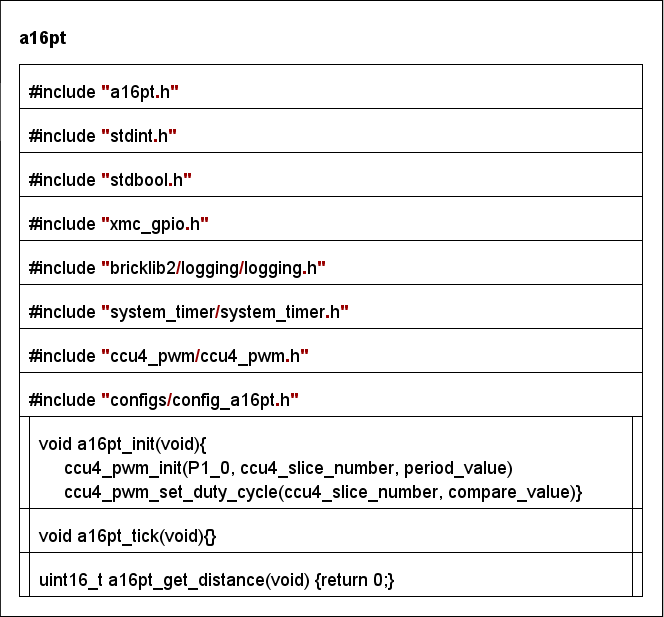
\includegraphics[width=1.0\textwidth]{Struktogramme/a16pt.png}\caption{Struktogramm der a16.pt}\label{fig:Bild2}
%\end{figure}
In der a16pt werden die für die Entfernungsmessung notwendigen Funktionen und die Interrupt anweisungen abgearbeitet, außerdem werden die Ein- und Ausgangsports hier geschaltet.\\
